% --
%
% Configuração do Documento
%
% --
\documentclass[10pt,brazil]{beamer}
\uselanguage{Portuguese}
\languagepath{Portuguese}
\usepackage[utf8]{inputenc}


% ---
% Pacotes adicionais
% ---
\usepackage[light,math]{kurier}         %Altera Fonte Utilizada no arquivo
\usepackage{amsmath,amsfonts,amsthm,amssymb,mathrsfs}
\allowdisplaybreaks[1]
\usepackage{microtype}
\usepackage{mathtools}
\usepackage{csquotes}
\usepackage{tikz}
\usetikzlibrary{matrix}
\usetikzlibrary{patterns}
\usepackage{faktor}
\usepackage[Sonny]{fncychap}
\usepackage{hyperref}
\usepackage{tikz}
\graphicspath{{images/}}
\usepackage[light,math]{kurier}
\usetheme{Madrid}
\useinnertheme{rectangles}


\renewcommand{\raggedright}{\leftskip=0pt \rightskip=0pt plus 0cm} %texto justificado

\usepackage[%
    alf,
    abnt-emphasize=bf,
    bibjustif,
    recuo=0cm,
    abnt-doi=expand,            % Expande um endereço iniciado com doi: para http://dx.doi.org/
    abnt-url-package=url,       % Utiliza o pacote url
    abnt-refinfo=yes,           % Utiliza o estilo bibliográfico abnt-refinfo
    abnt-etal-cite=3,
    abnt-etal-list=3,
    abnt-thesis-year=final
]{abntex2cite}   

\setbeamertemplate{theorems}[numbered] % to number
\setbeamercovered{transparent}

\theoremstyle{definition}
\newtheorem{dfn}{Definição}
\newtheorem{obs}{Observação}
\newtheorem*{proofthm}{Demonstração do Teorema}
\newtheorem*{proofprop}{Demonstração da Proposição}
\newtheorem{ex}{Exemplo}
\newtheorem{prop}{Propriedade}
\newtheorem{proposition}{Proposição}


\newcommand{\der}{\text{d}}					%Comando para fazer o d da derivada fora do ambienta matemático
\newcommand{\mb}[2]{\mathbb{#1}^{#2}}		%Comando para usar \mathbb de maneira  mais eficiente
\newcommand{\mca}[2]{\mathcal{#1}_{#2}}
\newcommand{\mul}[2]{\mu_{#1}\left(#2\right)}			%Comando para escrever a multiplicidade de modo mais eficiente
\newcommand{\mc}[2]{\mathcal{I}_{#1}\left(#2\right)}   %Comando para escrever o IPH de maneira  mais eficiente

% --
% Define Cores Personalizadas 
% --
\definecolor{ver}{RGB}{124,26,29}
\definecolor{yel}{RGB}{158,134,35}
\definecolor{ros}{RGB}{255,51,102}
\definecolor{ver1}{RGB}{169,88,99}
\definecolor{ver2}{RGB}{156,63,75}
\definecolor{ver3}{RGB}{145,43,56}
\definecolor{azul}{RGB}{18,35,97}

% --
% Customiza o título 
% --
\setbeamercolor{title}{fg=azul, bg=white!95!black}

% --
% Remove os controles de navegação 
% --
\setbeamertemplate{navigation symbols}{}

% --
% Customiza o background
% --
\setbeamertemplate{background}{
	\begin{tikzpicture}[remember picture,overlay]
	% --- LinhaInferior
	\draw[line width=0.4mm,azul] ([shift={(2.5cm,0.4cm)}]current page.south west) -- ([shift={(-0.38cm,0.4cm)}]current page.south east);
	\draw[line width=0.4mm,azul] ([shift={(-0.3cm,0.4cm)}]current page.south east) -- ([shift={(-0.26cm,0.4cm)}]current page.south east);
	\draw[line width=0.4mm,azul] ([shift={(2.75cm,0.3cm)}]current page.south west) -- ([shift={(-0.38cm,0.3cm)}]current page.south east);
	\draw[line width=0.4mm,azul] ([shift={(-0.3cm,0.3cm)}]current page.south east) -- ([shift={(-0.26cm,0.3cm)}]current page.south east);
	\draw[line width=0.4mm,azul] ([shift={(3cm,0.2cm)}]current page.south west) -- ([shift={(-0.38cm,0.2cm)}]current page.south east);
	\draw[line width=0.4mm,ver1] ([shift={(-0.3cm,0.2cm)}]current page.south east) -- ([shift={(-0.26cm,0.2cm)}]current page.south east);
	
	% --- Logo 
	\node[xshift=-1.5cm,yshift=-0.8cm] at (current page.north east) {
\includegraphics[scale=0.15]{logo_ufmg.jpg}};
	
	\end{tikzpicture}
}

% --
% Customiza o título do frame 
% --
\setbeamercolor{frametitle}{fg=azul, bg=white} 
\makeatletter
\setbeamertemplate{frametitle}
{
	\ifbeamercolorempty[bg]{frametitle}{}{\nointerlineskip}%
	\@tempdima=\textwidth%
	\advance\@tempdima by\beamer@leftmargin%
	\advance\@tempdima by\beamer@rightmargin%
	\pgfsetfillopacity{.1}       %<------ fix filling opacity
	\begin{beamercolorbox}[sep=0.3cm,left,wd=\the\@tempdima]{frametitle}
		\usebeamerfont{frametitle}%
		\vbox{}\vskip1ex \hskip6ex%
		\if@tempswa\else\csname beamer@fteleft\endcsname\fi%
		\strut\pgfsetfillopacity{1}\insertframetitle\strut\par%  <---- text opacity
		{%
			\ifx\insertframesubtitle\@empty%
			\else%
			{\usebeamerfont{framesubtitle}\usebeamercolor[fg]{framesubtitle}\insertframesubtitle\strut\par}%
			\fi
		}%
		\vskip-1ex%
		\if@tempswa\else\vskip-.3cm\fi% set inside beamercolorbox... evil here...
	\end{beamercolorbox}%
}
\makeatother


% --
% Customimza o ambiente de Teorema 
% --
\setbeamercolor{block title}{use=structure, fg=white, bg=azul}
\setbeamercolor{block body}{use=structure, fg=black, bg=white!96!black}
\setbeamertemplate{block begin}[default]
\setbeamertemplate{block end}[default]



% --
% Customiza o footline 
% --
\defbeamertemplate{footline}{centered page number}
{%
  \hspace*{\fill}%
  \usebeamercolor[fg]{page number in head/foot}%
  \usebeamerfont{page number in head/foot}%
  \insertpagenumber\,/\,\insertpresentationendpage%
  \hspace*{\fill}%
  \hspace*{\fill}%
  \hspace*{\fill}%
  \hspace*{\fill}%
  \hspace*{\fill}%
  \hspace*{\fill}%
  \hspace*{\fill}%
  \hspace*{\fill}%
  \hspace*{\fill}
  \hspace*{\fill}%
  \hspace*{\fill}%
  \hspace*{\fill}%
  \hspace*{\fill}\vskip6pt%
}
\setbeamertemplate{footline}[centered page number]

% --
% Customiza o headline 
% --
\setbeamertemplate{headline}
{
	\leavevmode%
	\hbox{%
		\begin{beamercolorbox}[wd=\paperwidth,dp=3.5ex]{ver}%
			\raggedright
			\hspace*{2em}%
		\end{beamercolorbox}%
	}%
}


% --
% Customiza o estilo dos ambientes Itemize e Enumerate 
% --
\setbeamertemplate{enumerate item}{\color{azul}\insertenumlabel)}
\setbeamertemplate{enumerate subitem}{\color{azul}\insertenumlabel.\insertsubenumlabel)}
\setbeamertemplate{enumerate subsubitem}{\color{azul}\insertenumlabel.\insertsubenumlabel.\insertsubsubenumlabel)}
\setbeamertemplate{enumerate mini template}{\insertenumlabel}

\setbeamertemplate{itemize item}{\scriptsize\raise1.25pt\hbox{\color{azul}\donotcoloroutermaths$\bullet$}}
\setbeamertemplate{itemize subitem}{\tiny\raise1.5pt\hbox{\color{azul}\donotcoloroutermaths$\blacksquare$}}
\setbeamertemplate{itemize subsubitem}{\tiny\raise1.5pt\hbox{\color{azul}\donotcoloroutermaths$\blacktriangleright$}}

% -- 
% Customiza o estilo do Table of Contents 
% --
\setbeamertemplate{section in toc}[square]

\setbeamerfont{section number projected}{size=\large}
\setbeamercolor{section number projected}{bg=white!95!black, fg=azul}

\setbeamertemplate{subsection in toc}{%
	\leavevmode\leftskip=5.65ex%
	\llap{\raisebox{0.2ex}{\textcolor{azul}{$\bullet$}}\kern1ex}%
	\inserttocsubsection\par%
}

% -- 
%Customiza as margens dos frames 
% -- 
\setbeamersize{text margin left=1cm,text margin right=1cm}

% -- 
% Apresentação
% -- 
\begin{document}
\mode<presentation>

% -- 
% Info
% -- 
\title[]{ANÁLISE DE DADOS UTILIZAND \emph{CLUSTER} E BAIXO CUSTO}
\subtitle{COMPARAÇÃO DE DESEMPENHO DE AMBIENTES VIRTUAIS}

\institute[UFMG]{Universidade Federal de Minas Gerais}

\author[Felipe Rocha]{Felipe Fonseca Rocha \\
  \vspace{0.25cm}
  Orientador: Ítalo Fernando Scotá Cunha}
\date{09 de Fevereiro de 2022}

% --
% Inclui o sumário antes de cada seção
% --
\AtBeginSubsection{%
  \begin{frame}
    \tableofcontents[currentsection,sectionstyle=show/shaded,subsectionstyle=show/hide/hide]
  \end{frame}
}
% -- 
% Cria slide com título
% -- 
\frame{\maketitle}

% -- 
% Cria slide com sumário
% -- 

\begin{frame}{Sumário}
  \tableofcontents[hideallsubsections]
\end{frame}

% 	\begin{figure}
% 		\centering
% 		\includegraphics[scale=0.45]{objetivo.jpg}
% 	\end{figure}

% --
%
% Conteúdo 
%
% --

% -- 
% Introdução
% -- 
\section{Contexto e Motivação}
% -- 
% Motivação
% -- 
\begin{frame}[allowframebreaks]{Contexto e Motivação}
  \begin{columns}
    \begin{column}{0.5\textwidth}
      \begin{itemize}
        \item[] A todo momento nós geramos milhões de dados que são coletados por diferentes meios
        \item[]
        \item[] Existem várias ferramentas disponíveis para transformá-los em informações e embasar decisões
      \end{itemize}
      %\cite{galvao_desafios_2019,mehta_concurrence_2018,brasildisponibilidade2016}
    \end{column}
    \begin{column}{0.5\textwidth}
      \begin{center}
        
\includegraphics[width=1\textwidth]{sis.png}
      \end{center}
    \end{column}
  \end{columns}
  \framebreak
  \begin{columns}
    \begin{column}{0.5\textwidth}
    \begin{center}
      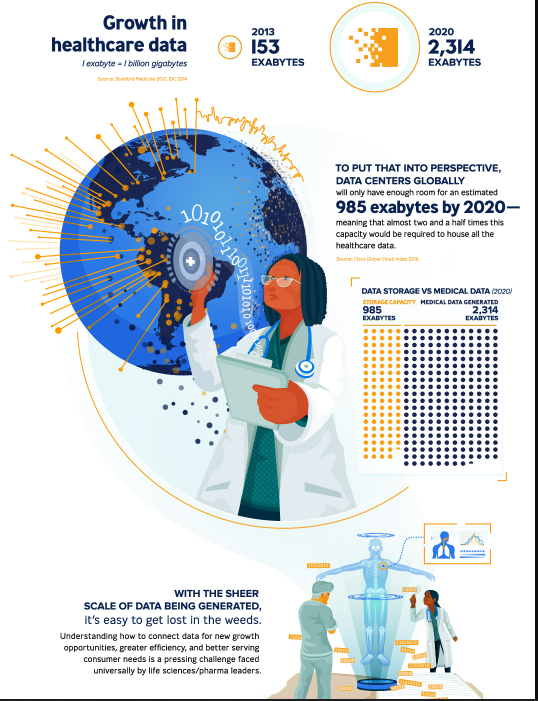
\includegraphics[width=.9\textwidth,height=.75\textheight]{growthhealth.png}
      \end{center}
    \end{column}
    \begin{column}{0.5\textwidth}
      \begin{itemize}
        \item[] Isso também acontece na área da saúde
        \item[]
        \item[] Porém o uso de ferramentas de \emph{big data} em saúde ainda é pouco significativo
        \item[]
        \item[] Boa parte dessas ferramentas implica processamento distribuído
      \end{itemize}
    \end{column}
  \end{columns}
  \framebreak
  \begin{columns}%\begin{center}
      \begin{column}{0.5\textwidth}
  \begin{itemize}
    \item[] Potencial de melhora do sistema de saúde através de análise de dados
    \item[]
    \item[] Integrar times com trabalho interdisciplinar
    \item[]
    \item[] Uso de ferramentas e recursos já disponíveis de maneira correta
    %item[] Plataformas de isolamento entre sistemas
  \end{itemize}
    \end{column}
    \begin{column}{0.5\textwidth}
      \begin{center}
        
\includegraphics[width=1\textwidth]{interdisciplinar.png}
      \end{center}
      \end{column}
   %\item Necessário propor e validar estratégias que sejam viáveis e facilitem o processamento de analise de grande volume de dados produzido na área
  \end{columns}
 %\end{center}
 %\framebreak
 % \begin{itemize}
 %   \item No Brasil, dados do Sistema de Informação em Sáude (SIS) são disponibilizados desde 2016
 %   \item \textbf{Faltam recursos} e estratégias viáveis para essa elaboração.
 % \end{itemize}
\end{frame}


\section{Justificativa}

% -- 
% Justificava
% -- 
\subsection{Justificativa Social}

\begin{frame}{Justificativa Social}

      \begin{itemize}
            \item Tomada de decisão em saúde
            \item Escala: $152$ \textbf{milhões} dependem exclusivamente do SUS
            \item Restrição: Gasto de $R\$3.83$ por pessoa por dia
            \item Volume de dados disponibilizados 
            \item \textbf{Assertividade}
      \begin{itemize}
          \item Ações em saúde
          \item políticas publicas
      \end{itemize}
      \end{itemize}
 
\end{frame}

\subsection{Justificativa Econômica}

\begin{frame}{Justificativa Econômica}
  \begin{columns}
    \begin{column}{0.5\textwidth}
              \begin{itemize}
                \item Gasto na disponibilização dos dados
                \item Diminuição de verbas para ciência e tecnologia -$2,32\%$
      \end{itemize}
    \end{column}
    \begin{column}{0.5\textwidth}  %%<--- here
      \begin{center}
        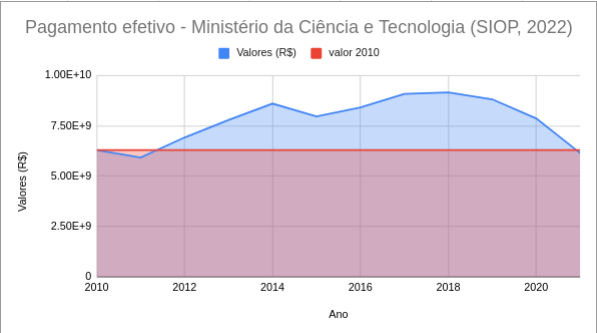
\includegraphics[width=1\textwidth]{orcamento.png}
        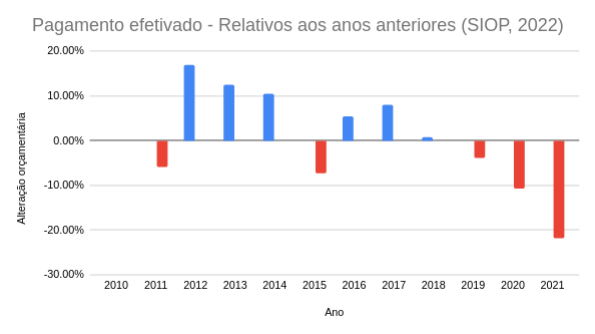
\includegraphics[width=1\textwidth]{variacaoorcamentaria.png}
      \end{center}
    \end{column}
  \end{columns}
\end{frame}

\begin{frame}{Justificativa Econômica}
  \begin{columns}
    \begin{column}{0.5\textwidth}
      \begin{itemize}
            \item Aumento do dólar em mais de $327\%$ diminuindo o poder de compra
            \item Aumento do custo de hardware e máquinas
      \end{itemize}
    \end{column}
    \begin{column}{0.5\textwidth}  %%<--- here
      \begin{center}
        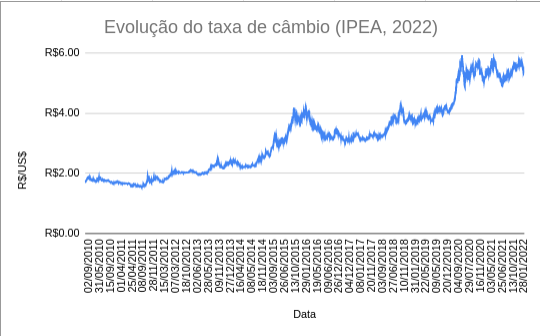
\includegraphics[width=1\textwidth]{variacaodolar.png}        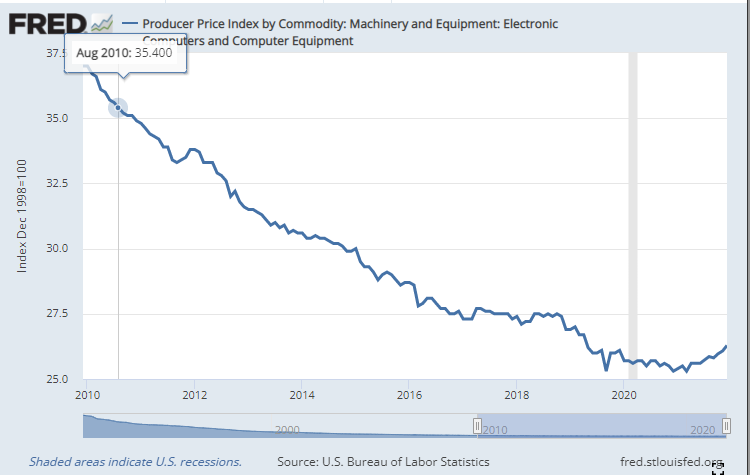
\includegraphics[width=1\textwidth]{hardwarecost.png}
      \end{center}
    \end{column}
  \end{columns}
\end{frame}

\subsection{Justificativa Técnica}

\begin{frame}{Justificativa Técnica}
  \begin{columns}
    \begin{column}{0.5\textwidth}
      \begin{itemize}
            \item Necessário ser interdisciplinar
            \item Avaliar alternativas de processamento de dados 
            \item Amenizar questões orçamentárias
            \item Melhorar uso dos recursos já existentes
      \end{itemize}
  \end{column}
    \begin{column}{0.5\textwidth}  %%<--- here
      \begin{center}
        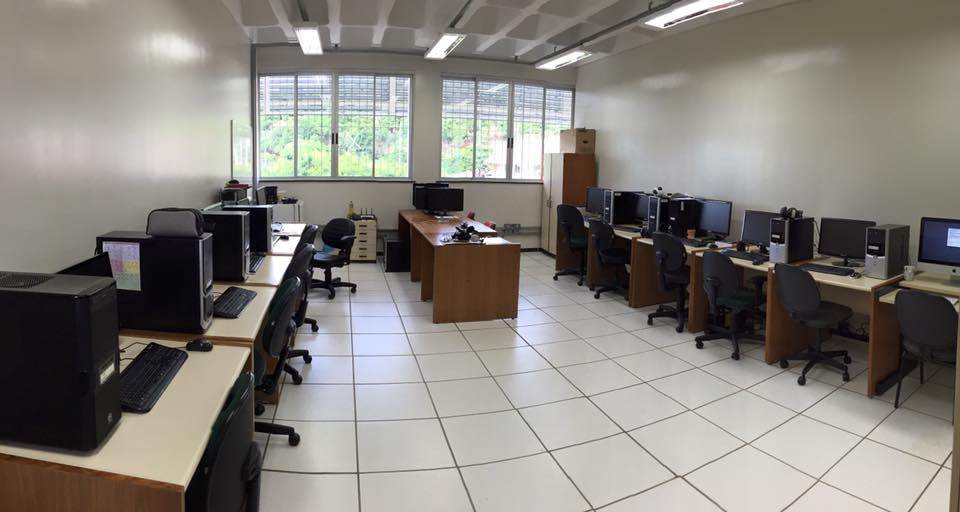
\includegraphics[width=1\textwidth]{lab.jpg}        
        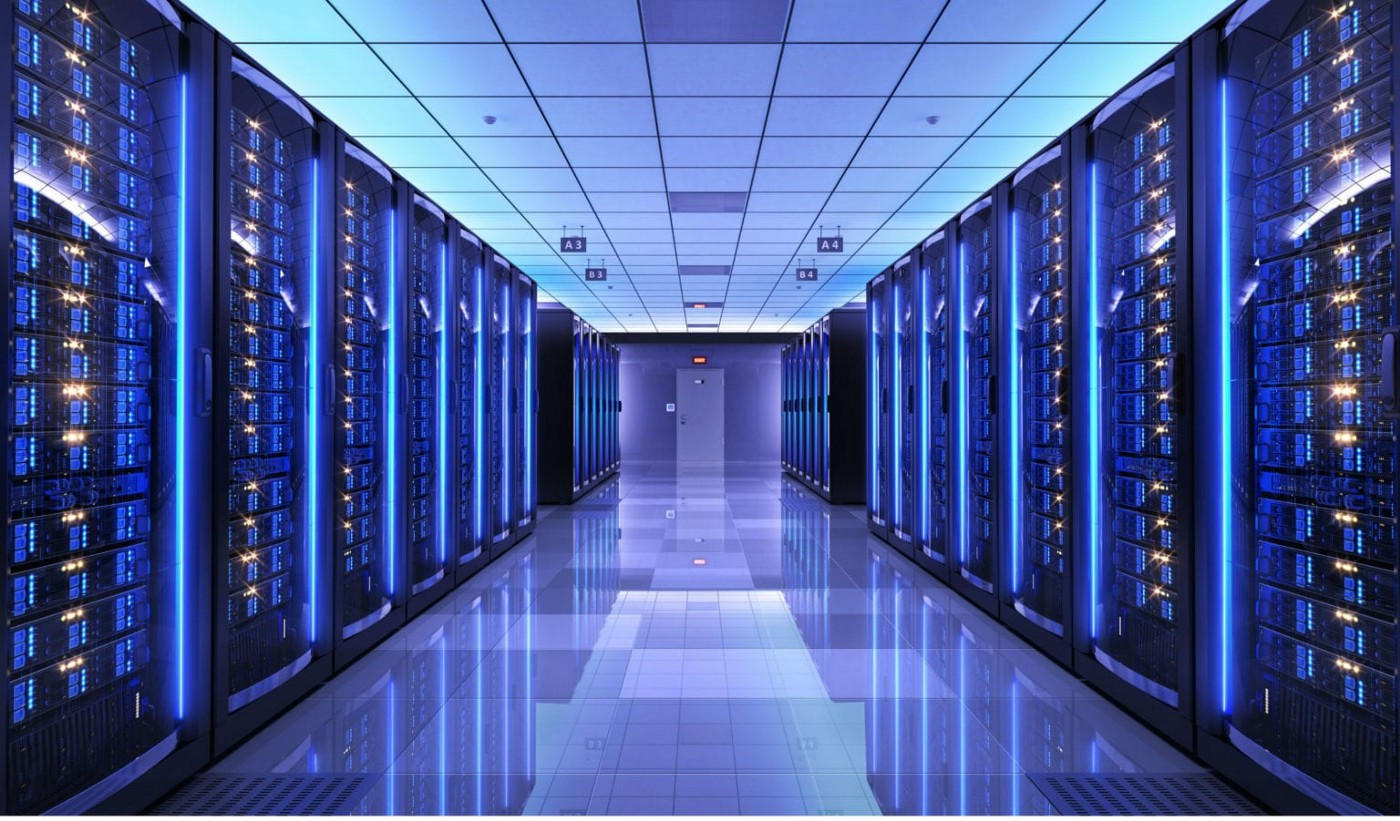
\includegraphics[width=1\textwidth]{hpc.jpeg}        
      \end{center}
    \end{column}
  \end{columns}
\end{frame}


% -- 
% Objetivos
% -- 
\section{Objetivo}
%[allowframebreaks]
\begin{frame}[allowframebreaks]{Objetivo}
  \begin{itemize}
    \item[] \textbf{Objetivos Geral:}
    \item[]
          \begin{itemize}
            \item[] Realizar a comparação de desempenho de orquestração de recursos em \emph{cluster} de baixo custo em ambientes virtualizados, para o processamento e a análise dos dados.
          \end{itemize}
    \item[] \textbf{Objetivos Específicos:}
          \begin{itemize}
            \item Realizar a orquestração de recursos em \emph{cluster} de baixo custo;
            \item Comparar o desempenho de \emph{clusters} bem ambientes virtualizados;
            \item Validar o uso de um \emph{cluster} de utilização compartilhada para processamento de dados distribuídos;
            \item Propor um método de análise em \emph{cluster} Kubernetes com uso de computadores desktops;
          \end{itemize}
          I\end{itemize}
\end{frame}


% -- F
% Revisão de Literatura
% -- 
\section{Revisão de literatura}

% -- 
%  Análise de dados
% -- 
\subsection{Análise de dados}

\begin{frame}{Análise de dados}
  \begin{itemize}
    \item Descisões em saúde costumam ser complexas - precisam de suporte científico (dados) e avaliação de Contexto
    \item Com o crescimento dos 3V's de dados na área da saúde (Big Data) processar e analisar esses dados tornouse fundamental para tomada de descisões adequadas
    \item Desafios:
          \begin{itemize}
            \item complexidade dos dados obtidos
            \item ausencia de validação de sistemas, métodos e ferramentas para o tratamento de dados na área
            \item custos de novos equipamentos capazes de analisar tal volume
          \end{itemize}
    \item Há grande oportunidade para a proposição de estratégias de processamento e anális de dados na área
  \end{itemize}
\end{frame}

% -- 
%  Alternativas open source
% -- 
\subsection{Alternativas \emph{open source}}

\begin{frame}{Alternativas \emph{open source}}
  \begin{itemize}
    \item Considerando
          \begin{itemize}
            \item O escopo deste trabalho
            \item As estratégias para processamento e análise de dados disponíveis no mercado
          \end{itemize}
    \item [] As soluções encontradas no mercado foram agrupadas em dois grupos:
          \begin{itemize}
            \item Soluções de Computação em nuvem privada:
                  \begin{itemize}
                    \item Se estendem para além do proposito desse trabalho
                    \item Requisitos de hardware elevados
                    \item Complexidade de configuração devido a sua abrangência
                  \end{itemize}
          \end{itemize}
  \end{itemize}
\end{frame}


\begin{frame}{Alternativas \emph{open source}}
  \begin{columns}
    \begin{column}{0.5\textwidth}
      \begin{itemize}
        \item Soluções de Orquestração de Containers:
              \begin{itemize}
                \item Kubernetes\textregistered
                \item Apache Mesos\textregistered
                \item Hashicorp Nomad\textregistered\*
                \item Docker Swarm\textregistered
              \end{itemize}
      \end{itemize}
    \end{column}
    \begin{column}{0.5\textwidth}  %%<--- here
      \begin{center}
        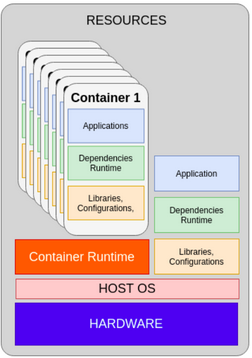
\includegraphics[width=0.5\textwidth]{containers.png}
        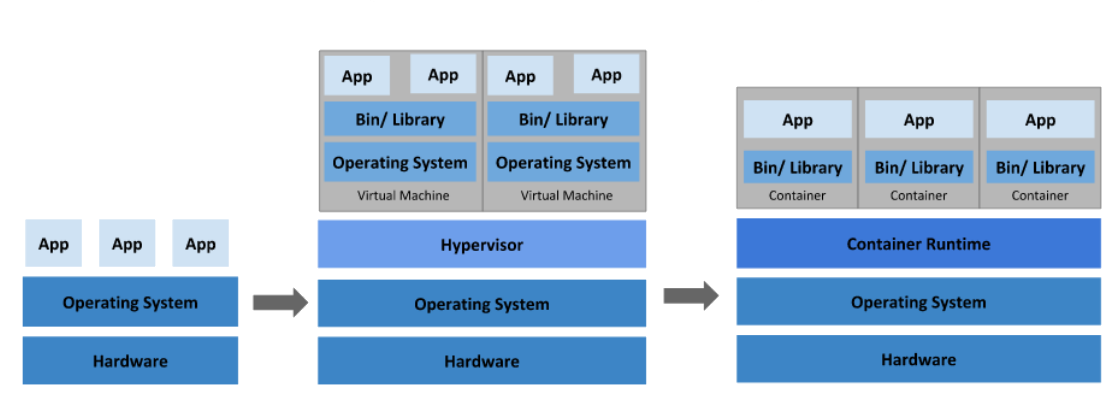
\includegraphics[width=1\textwidth]{vmsContainer.png}
      \end{center}
    \end{column}
  \end{columns}
\end{frame}

% -- 
% \emph{Cluster}orquestrador de container
% -- 
\subsection{Cluster orquestrador de container}

\begin{frame}{Cluster orquestrador de container}
  \begin{columns}
    \begin{column}{0.5\textwidth}
      \begin{itemize}
        \item Kubernetes\textregistered:
              \begin{itemize}
                \item Origem de 15 anos de trabalho da Google (Borg) %\cite{verma_large-scale_2015}
                \item Estrutura de objetos componentizados %\cite{kubernetes2022}
                      \begin{itemize}
                        \item Kube-apiserver
                        \item Kube-scheduler
                        \item Kube-controller-manager
                        \item Kubelet
                        \item Kube-proxy
                        \item Pod
                      \end{itemize}
              \end{itemize}
      \end{itemize}
    \end{column}
    \begin{column}{0.5\textwidth}  %%<--- here
      \begin{center}
        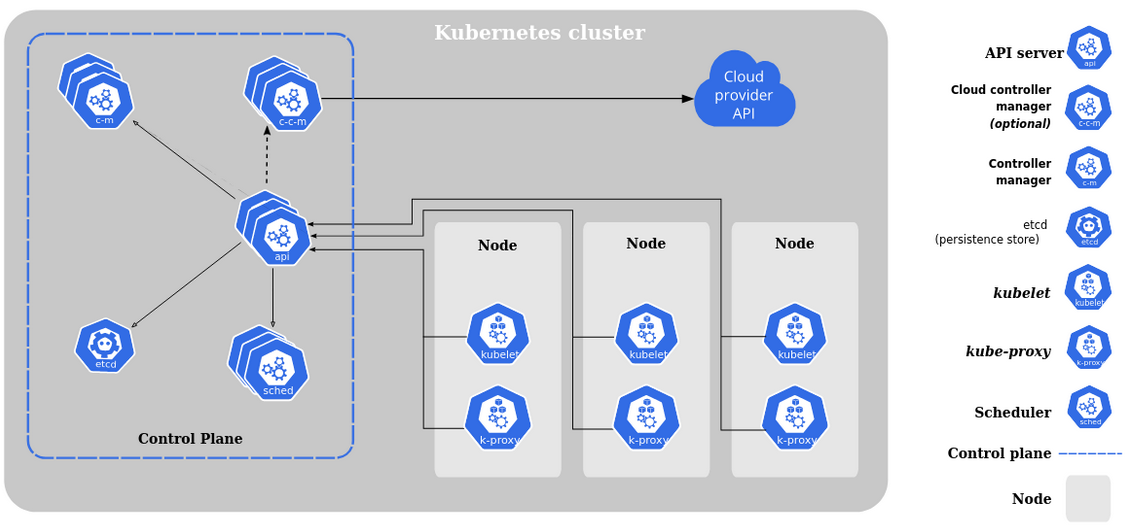
\includegraphics[width=1\textwidth]{kubeadm-node.png}
      \end{center}
    \end{column}
  \end{columns}
\end{frame}

% -- 
% Métodos
% -- 
\section{Método}

% -- 
% Abordagem
% --
\subsection{Abordagem}
\begin{frame}[allowframebreaks]{Abordagem}
  Utilizar u \emph{Cluster} ubernetes como plataforma de orquestração de cargas de trabalho em ambiente virtual.
  \begin{itemize}
    \item Cargas de trabalho:
          \begin{itemize}
            \item Analise de tendencia de uso de azitromicina entre 2014 e 2021
          \end{itemize}
        \item Ambientes virtualizados (\emph{Host} do cluster):
          \begin{itemize}
            \item completa - \emph{Hypervisor} tipo 2
            \item sistema operacional - contêineres
        \end{itemize}
    
        \item máquinas subutilizadas
        \item redução do CAPEX
    \end{itemize}
\end{frame}

\begin{frame}{Abordagem}
  O uso de conceitos e metodologias de DevOps:
  \begin{itemize}
            \item CI (integração contínua)
            \item CD (entrega contínua)
    \item Monitoramento
        \begin{itemize}
            \item método USE, parâmetros de utilização, saturação e erro 
            \item métricas definidas por parâmetro
            \item relaciona desempenho dos nós virtuais.
        \end{itemize}
  \end{itemize}
\end{frame}

% -- 
% Especificação dos nós integrantes \emph{cluster} 
% -- 
\subsection{Especificações}

\begin{frame}[allowframebreaks]{Especificações}
  \begin{columns}
    \begin{column}{0.5\textwidth}
      \begin{itemize}
        \item Cluster:
              \begin{itemize}
                \item Virtualização:
                      \begin{itemize}
                        \item Maquinas Virtuais (VMs) (\emph{Hypervisor} tipo 2)
                        \item Contêineres Aninhados (Docker In Docker, ou DinD)
                      \end{itemize}
              \end{itemize}
        \begin{itemize}
            \item Ambiente Virtual:
              \begin{itemize}
              \item  arquitetura: \textbf{amd64}
                \item 1 vCPU
                \item 2 GB de RAM
                \item 6-8 máquinas
              \end{itemize}
        \end{itemize}
    \end{itemize}
    \end{column}
    \begin{column}{0.5\textwidth}  %%<--- here
      \begin{center}
        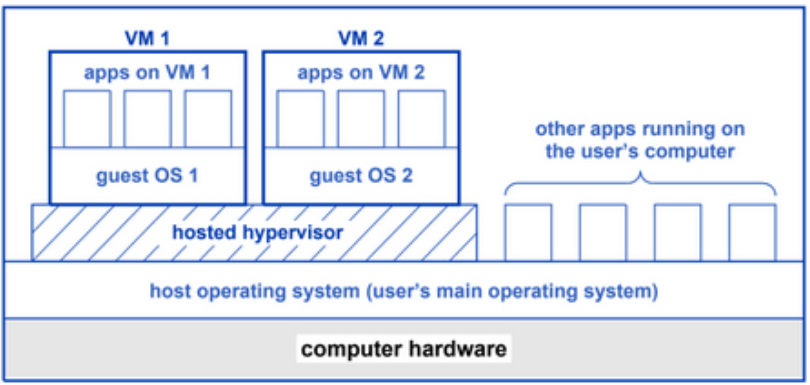
\includegraphics[width=1\textwidth]{vms.png}
      \end{center}
    \end{column}
  \end{columns}
  
  \framebreak
  
  \begin{columns}
    \begin{column}{0.5\textwidth}
    
      \begin{itemize}
        \item Definição máquina \emph{host}:
              \begin{itemize}
                \item o \emph{host} será um laptop, contendo configuração de 4vCPUs e 16GB de RAM
                \item Hospedará as maquinas virtualizadas, pertencentes ao cluster
                      
              \end{itemize}
        \item Definição máquina \emph{guest}:
              \begin{itemize}
                \item como ja descrtio em 2 cenários: Virtualização completa, e em containers
                \item Nós d \emph{Cluster} ubernetes (objeto de monitoramento)
              \end{itemize}
      \end{itemize}
    \end{column}
    \begin{column}{0.5\textwidth}
      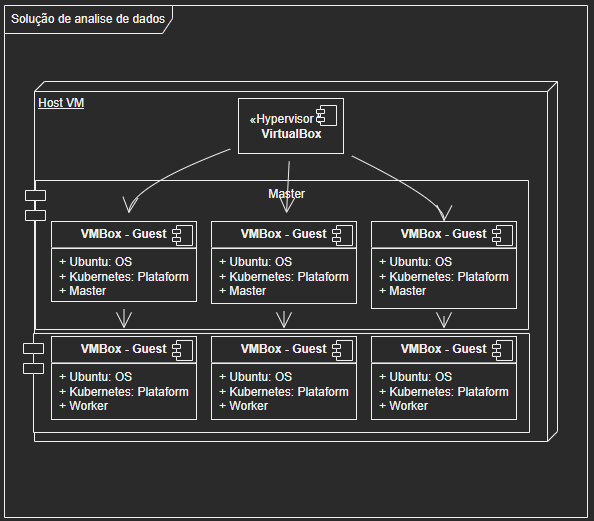
\includegraphics[width=1\textwidth]{SCKET.png}
    \end{column}
  \end{columns}
\end{frame}


% -- 
% Plataforma de orquestração de carga de trabalho
% -- 
\subsection{Arquitetura Orquestrador}

\begin{frame}{Arquitetura Orquestrador}
\begin{figure}
    \centering
    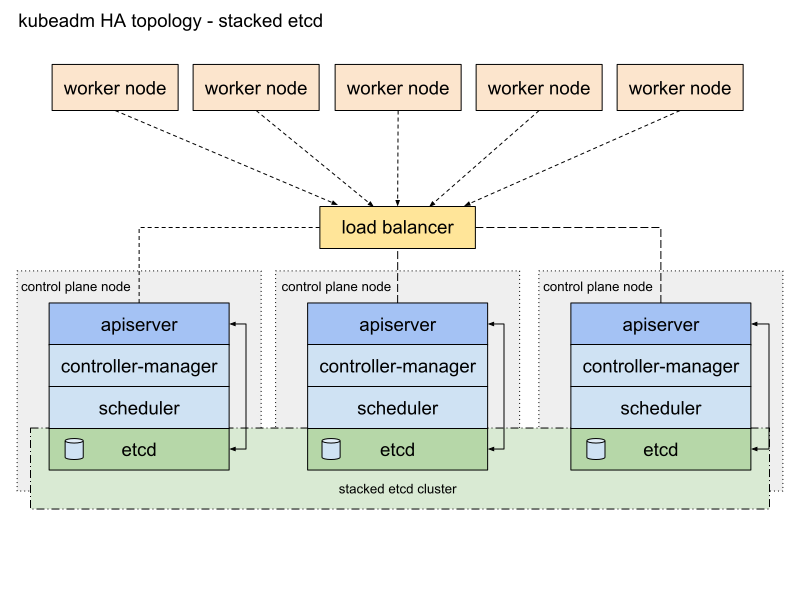
\includegraphics[width=1\textwidth]{kubeadm-ha-topology-stacked-etcd.png}
    %\caption{Caption}
    \label{fig:k8s-arch}
\end{figure}
\end{frame}
% -- 
% Configuração e provisionamento do cluster
% -- 
\subsection{Gerenciamento de configuração}

\begin{frame}{Gerenciamento de configuração}
      \begin{figure}
          \centering
      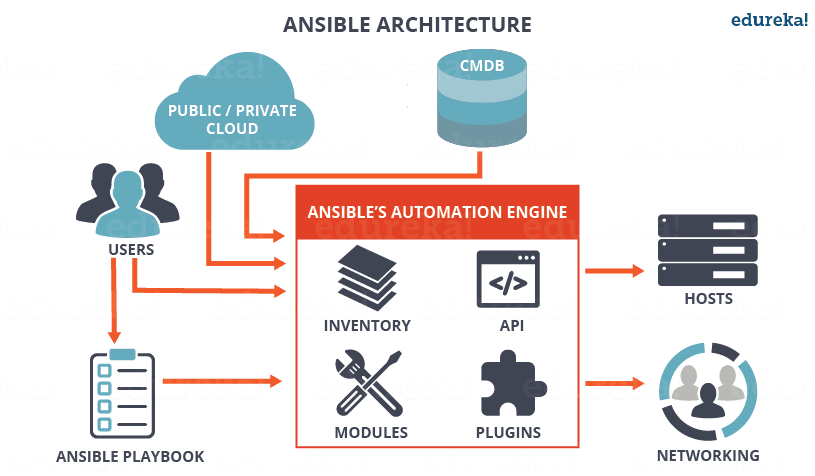
\includegraphics[width=.8\textwidth]{ansible arch.png}
          %\caption{Caption}
          \label{fig:ansiblearch}
      \end{figure}
      
\end{frame}

% -- 
% Monitoramento
% -- 
\subsection{Monitoramento}

\begin{frame}{Monitoramento}
  \begin{itemize}
    \item \emph{OpenTelemetry}
    \item \emph{Prometheus} Monitoramento de sistemas e Banco de dados de series temporais
    \item \emph{Grafana} - Dashboard e observabilidade
    \item Parametros de tempo, taxa de utilização de memoria e processamento
  \end{itemize}
\end{frame}


% -- 
% Comparação entre tipos de virtualização
% -- 
\subsection{Comparação entre tipos de virtualização}

\begin{frame}[allowframebreaks]{Comparação entre tipos de virtualização}
  
  \begin{itemize}
      \item macrobenchmark (system level benchmark) - Teste utizando uma solução avaliando tempo de execussão
      \item[] métricas de Desempenho (nós do cluster, \emph{guests}):
      \item Taxa de Utilização de CPU e Memória 
      \item Taxa de saturação de CPU e Memória
      \item[] Métricas de APM:
      \item Tempo Médio de todas as cargas de trabalho e variabilidade
      \item[] Método base utilizado para coleta de informações:
      \item Metodo USE de avaliação (Checklist Linux)
  \end{itemize}
  
  Caso base - comparação com processo de análise em \emph{bare metal} 4vCPU, 16 GB de RAM - totalizando o poder computacional total do \emph{cluster} proposto
\end{frame}


% -- 
% Análise de dados
% -- 
\subsection{Análise de dados}

\begin{frame}{Exemplo da Análise de dados}
  \begin{itemize}
    \item Vendas de Medicamentos Controlados e Antimicrobianos - Medicamentos Industrializados
    \item $530 \cdot 10^{6}$ linhas com mais de 70 GB
    \item Análise de tendência do consumo de azitromicina
  \end{itemize}
\end{frame}

% -- 
% Cronograma
% -- 
\subsection{Cronograma}

\begin{frame}[plain]
  \hspace*{-10mm}
  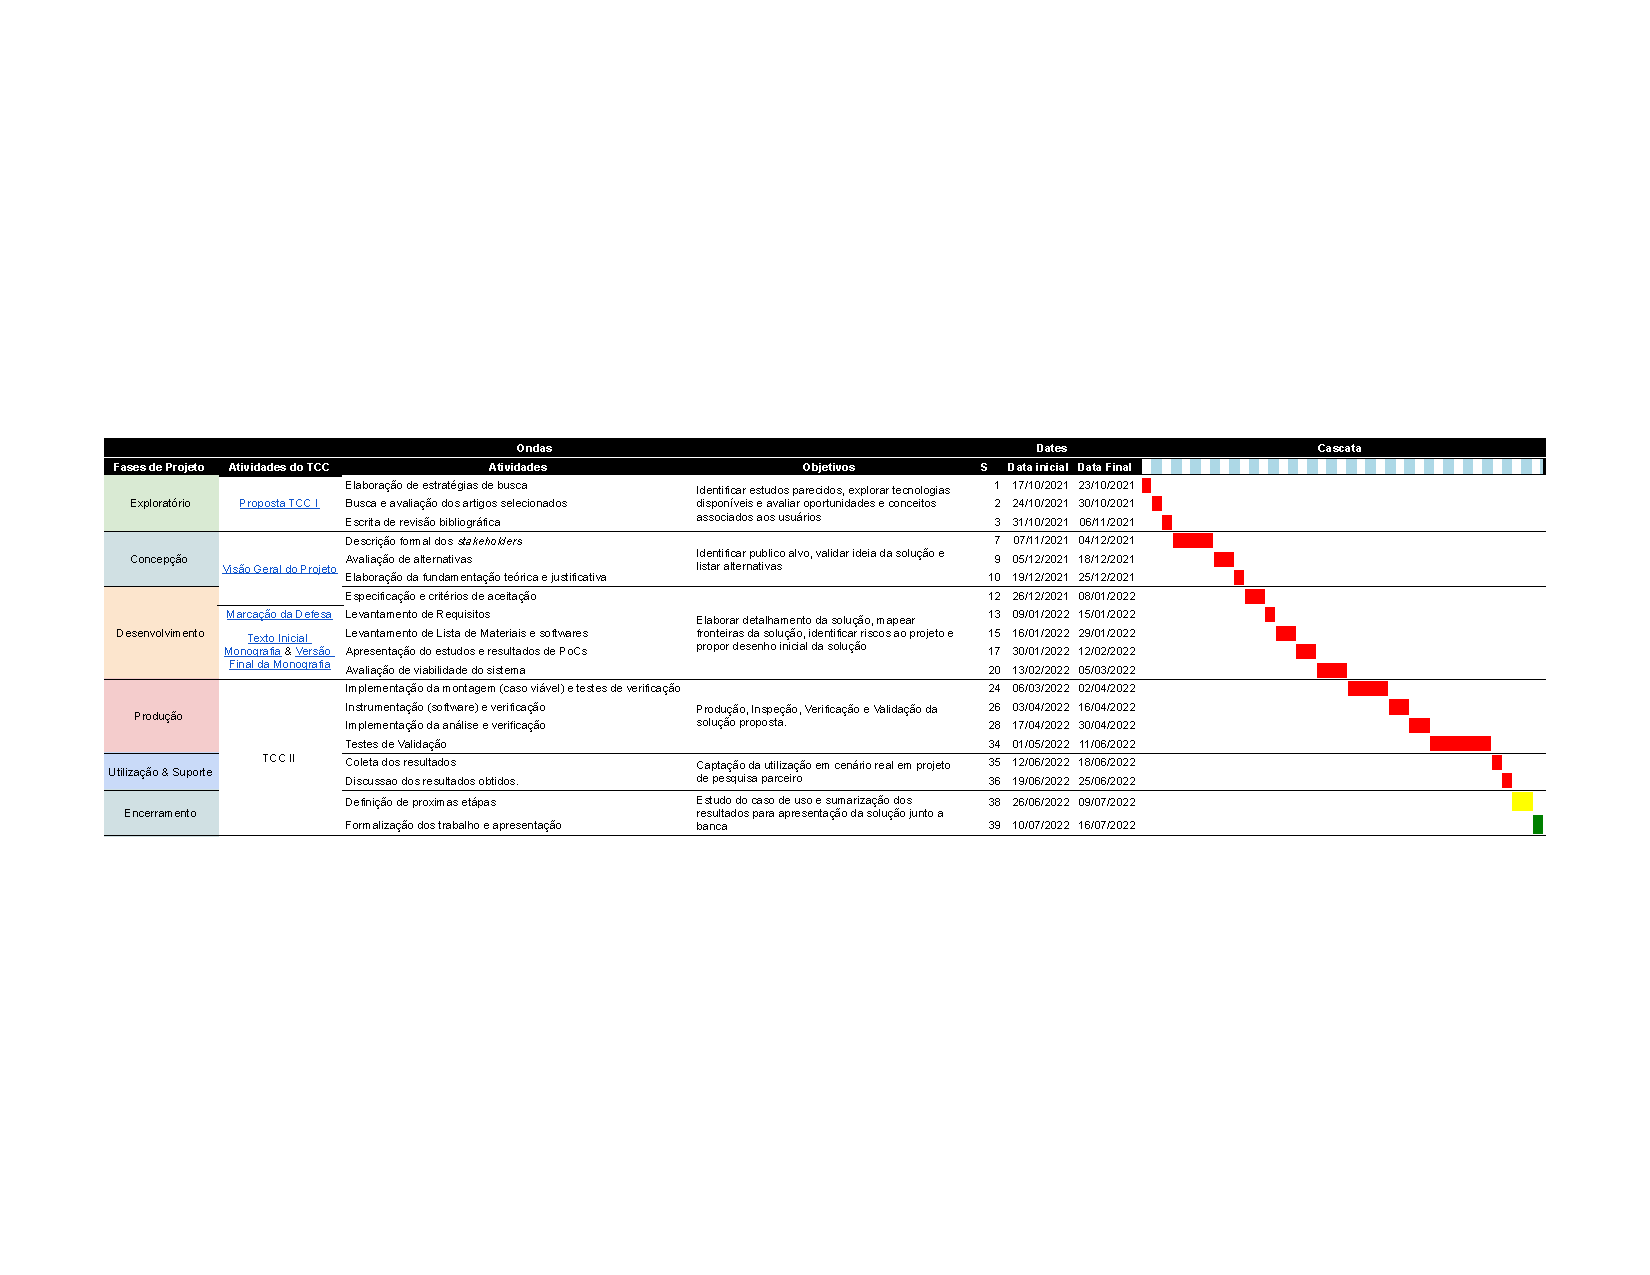
\includegraphics[width=\paperwidth]{TCC cronograma - Sheet1.pdf}
\end{frame}

% -- 
% Conclusão
% -- 
\section{Conclusão}

\begin{frame}{Conclusão}
  \begin{itemize}
    \item Entendimento da complexidade dos fatores considerados no processo de decisão em saúde
    \item Análise dos impactos sociais-econômicos relativos a restrição orçamentária na ciência
    \item Seleção de tecnologias com base em requisitos e restrições
    \item Desenho de uma estratégia de extração de informações em saúde
    \item Avaliação de diferentes tipos de virtualização e sua utilização
  \end{itemize}
  Trabalhos futuros contemplarão a implementação, testes e coletas de dados para avaliação comparativa das virtualizações propostas. 
  
  Baseado nesses resultados pode se evoluir essa discussão na forma de recrutamento de computadores para o \emph{cluster} de maneira a garantir o isolamento da maquina base.
\end{frame}


% -- 
% Disponibilidade dos recursos deste trabalho
% -- 
\section{Disponibilidade dos recursos deste trabalho}

\begin{frame}{Disponibilidade dos recursos deste trabalho}
  \begin{itemize}
    \item \href{https://github.com/felipefrocha/esufmg-tcc}{Github - Monorepo}
    \item \href{https://github.com/felipefrocha/esufmg-tcc/actions}{Pipeline}
  \end{itemize}
  Todos os componentes definidos neste trabalho estarão contidos em um ou mais repositórios públicos, sob a licença pública geral GNU versão 3, para livre acesso.
  
\end{frame}

% -- 
% Referências
% -- 
\begin{frame}[allowframebreaks]{Referências}
  \small
  %	\nocite{*}
  %    \bibliographystyle{apalike}
  \bibliography{Apresentacao}
\end{frame}


\begin{frame}
  \centering
  {\color{ros} OBRIGADO\\
    :)}
\end{frame}
\end{document}